\documentclass[conference]{IEEEtran}
\IEEEoverridecommandlockouts
\usepackage{cite}
\usepackage{amsmath,amssymb,amsfonts}
\usepackage{algorithmic}
\usepackage{graphicx}
\usepackage{textcomp}
\usepackage{xcolor}
\def\BibTeX{{\rm B\kern-.05em{\sc i\kern-.025em b}\kern-.08em
    T\kern-.1667em\lower.7ex\hbox{E}\kern-.125emX}}

\begin{document}

\title{Spatio-Temporal ConvLSTM for Cellular Traffic Forecasting: A Deep Learning Benchmark on the Telecom Italia Milan Dataset}


\author{
\begin{tabular}{cc}

\begin{tabular}{c}
\IEEEauthorblockN{Aarav Raj Shrestha}
\IEEEauthorblockA{
\textit{Department of Computer Science and Engineering}\\
AP23110011302
}
\end{tabular}
&
\begin{tabular}{c}
\IEEEauthorblockN{Maram Hasini Sai}
\IEEEauthorblockA{
\textit{Department of Computer Science and Engineering}\\
AP23110010502
}
\end{tabular}
\\[0.6cm]

\begin{tabular}{c}
\IEEEauthorblockN{Anjali Desai}
\IEEEauthorblockA{
\textit{Department of Computer Science and Engineering}\\
AP23110010509
}
\end{tabular}
&
\begin{tabular}{c}
\IEEEauthorblockN{Baibhav Baidya}
\IEEEauthorblockA{
\textit{Department of Computer Science and Engineering}\\
AP23110010756
}
\end{tabular}

\\[0.6cm]

\multicolumn{2}{c}{
\begin{tabular}{c}
\IEEEauthorblockN{Ajay B}
\IEEEauthorblockA{
\textit{Faculty Guide}\\
\textit{Department of Computer Science and Engineering}\\
SRM University-AP\\
ajay.b@srmap.edu.in
}
\end{tabular}
}

\end{tabular}
}

\maketitle

\begin{abstract}
Anticipating short-term cellular traffic demand is vital for dynamic radio resource allocation, automated antenna tilting, proactive edge caching, and energy-aware base station sleep scheduling in next-generation 5G and 6G cellular networks. Cellular traffic exhibits complex spatial inter-dependencies across urban neighborhoods as well as non-linear temporal rhythms driven by human activity. In this paper, we formulate short-term cellular internet traffic forecasting across an entire metropolitan area as a spatio-temporal video prediction task. We design and evaluate a two-layer Convolutional Long Short-Term Memory (ConvLSTM) neural network equipped with cyclical calendar encodings and a multi-scale residual prediction head. The model is benchmarked on the full-scale Telecom Italia Big Data Challenge dataset for Milan, comprising 62 consecutive days of telecommunications activity across a $100 \times 100$ spatial grid (10,000 cells) at 10-minute temporal granularity. To prevent data leakage, we enforce a strict chronological 70/15/15 train-validation-test split, with scaling parameters computed exclusively on the training partition. Through iterative engineering across three complete training regimes, we demonstrate that coupling logarithmic variance stabilization with standardization achieves superior relative accuracy. Evaluated on an out-of-distribution holiday test set (Christmas to New Year), our proposed model achieves a Root Mean Square Error (RMSE) of 8.4722, Mean Absolute Error (MAE) of 3.7802, and Mean Absolute Percentage Error (MAPE) of 10.585\%, outperforming the strongest persistence baseline by 9.80\% in RMSE, 12.79\% in MAE, and 15.73\% in MAPE, while substantially outperforming historical window averaging and seasonal benchmarks.
\end{abstract}

\begin{IEEEkeywords}
Cellular traffic forecasting, Spatio-temporal deep learning, Convolutional LSTM, Mobile network optimization, Telecom Italia dataset, Video frame prediction.
\end{IEEEkeywords}

\section{Introduction}
Modern cellular communication systems operate under highly volatile spatial and temporal demand patterns. Rapid urbanization, the pervasive adoption of mobile streaming and smart devices, and localized congregation events (such as sporting events, concerts, or commuting transit surges) cause rapid fluctuations in traffic density across metropolitan cellular grids \cite{b1}. Conventional cellular management paradigms rely on reactive adjustments, in which network controllers trigger power allocation, beam-steering, or handover handshakes only after localized congestion or packet queuing has already degraded service quality. In contrast, proactive network resource management seeks to predict traffic volume minutes or hours ahead of time. Accurate short-term predictions enable proactive beamforming, dynamic bandwidth re-allocation, preemptive edge server caching, and green base-station sleep cycling, yielding substantial operational expenditure and energy savings \cite{b2}.

Cellular traffic displays dual characteristics:
\begin{enumerate}
    \item \textbf{Spatial Correlation:} Telecommunication activity in a given cellular coverage area is strongly coupled to its geographical surroundings. Pedestrian and vehicular movement transfers demand across contiguous cells along arterial avenues and transit corridors.
    \item \textbf{Temporal Dynamics:} Cellular traffic exhibits prominent daily (diurnal) cycles, weekly periodicities (workdays vs. weekends), and short-term autoregressive inertia.
\end{enumerate}

Traditional statistical time-series models, such as Auto-Regressive Integrated Moving Average (ARIMA) and Holt-Winters exponential smoothing, model temporal autoregression on isolated single-cell time series but discard spatial spatial correlations across neighboring cells \cite{b3}. Conversely, standard Feedforward Convolutional Neural Networks (CNNs) process 2D spatial feature maps effectively but lack recurrent memory mechanisms to capture time-dependent evolutions. Standard Recurrent Neural Networks (RNNs) and Long Short-Term Memory (LSTM) networks require spatial grids to be flattened into 1D vectors, thereby destroying 2D topological adjacencies and inducing parameter explosion.

To jointly model spatial topology and temporal evolution, Shi et al. \cite{b4} introduced the Convolutional LSTM (ConvLSTM) for precipitation nowcasting from radar imagery. By treating a metropolitan cellular network as a 2D image where pixel intensities represent aggregated traffic and stacking consecutive observations as a video sequence, cellular traffic forecasting can be formulated as a spatio-temporal video frame prediction problem \cite{b5}.

In this paper, we develop, optimize, and rigorously benchmark an end-to-end Spatio-Temporal ConvLSTM architecture for 10-minute-ahead cellular internet traffic forecasting across the entire metropolitan area of Milan. Our core contributions are:
\begin{itemize}
    \item \textbf{Full-Scale, Leakage-Free Pipeline:} We process the entire 62-day, 20.8\,GB Telecom Italia Big Data Challenge dataset (8,928 consecutive 10-minute intervals over 10,000 spatial cells), enforcing strict chronological splitting and train-only normalization to prevent temporal and spatial data leakage.
    \item \textbf{Engineered Architecture:} We construct a deep recurrent network comprising two stacked ConvLSTM layers paired with sinusoidal cyclical calendar encodings and a residual convolutional refinement prediction head.
    \item \textbf{Iterative Methodological Optimization:} We document the progression across three full-scale training regimes, demonstrating how transition from min-max normalization to standard scaling and finally logarithmic variance-stabilizing transformation ($\log(1+x)$) overcomes gradient vanishing and reduces Mean Absolute Percentage Error (MAPE) by 11.7\%.
    \item \textbf{Comprehensive Benchmarking:} We benchmark our model against four baseline strategies—Persistence, Window Mean, Seasonal Daily, and Seasonal Weekly—demonstrating statistically significant improvements across an out-of-distribution holiday test window.
\end{itemize}

\section{Related Work}

\subsection{Statistical and Classical Machine Learning Approaches}
Early cellular traffic prediction studies utilized classical statistical models such as ARIMA, SARIMA, and Vector Auto-Regression (VAR) \cite{b3}, \cite{b6}. While mathematically tractable, these models assume linear Gaussian dynamics and cannot scale to high-dimensional spatial grids ($N = 10,000$). Support Vector Regression (SVR) and Random Forests introduced non-linear modeling capabilities but require extensive handcrafted feature engineering and struggle to preserve spatial continuity.

\subsection{Deep Learning for Spatial and Temporal Modeling}
The advent of deep learning popularized two distinct paradigms:
\begin{itemize}
    \item \textbf{Temporal Architectures:} Standard LSTMs \cite{b7} and Gated Recurrent Units (GRUs) effectively mitigate the vanishing gradient problem in long sequence modeling. However, applying them to spatial grids requires flattening $100 \times 100$ cells into a 10,000-dimensional vector, destroying spatial inductive biases and requiring tens of millions of fully connected weights.
    \item \textbf{Spatial Architectures:} Deep CNN architectures (e.g., ST-ResNet \cite{b8}) process spatial grids by treating past time intervals as static stacked input channels. Although spatial neighborhoods are preserved, the temporal dynamics are collapsed into fixed convolutional filters without recurrent memory states.
\end{itemize}

\subsection{Spatio-Temporal Recurrent Networks}
The ConvLSTM framework \cite{b4} unified spatial convolutions with recurrent state transitions by replacing standard matrix multiplications in the LSTM cell with convolutional operators. Subsequent extensions include PredRNN \cite{b9}, which introduced zig-zag memory flow, and Graph Convolutional Networks (GCNs) combined with GRUs \cite{b10} for irregular sensor topologies. For uniformly discretized urban grids, ConvLSTM remains the gold standard owing to its spatial parameter sharing, translational equivariance, and computational efficiency.

\subsection{Literature Gaps on the Telecom Italia Dataset}
While numerous papers evaluate on the Telecom Italia Milan dataset \cite{b11}, \cite{b12}, many prior works exhibit critical methodological limitations:
\begin{enumerate}
    \item \textbf{Data Leakage:} Shuffling sliding windows randomly across the temporal horizon leaks future observations into the training set, artificially inflating accuracy.
    \item \textbf{Spatial Sub-sampling:} Many studies restrict their evaluation to an arbitrary central $20 \times 20$ subgrid, bypassing peripheral cellular dynamics.
    \item \textbf{Weak Baselines:} Failing to compare against the highly competitive Persistence baseline (predicting the latest observed frame), which is notoriously difficult to outperform in 10-minute short-term forecasting.
\end{enumerate}
Our work addresses each of these gaps systematically.

\section{Dataset and Problem Formulation}

\subsection{Dataset Overview}
The dataset is drawn from the Telecom Italia Big Data Challenge \cite{b11}, \cite{b12}, capturing telecommunications activity in Milan, Italy, from November 1, 2013 to January 1, 2014 (62 consecutive days). 
\begin{itemize}
    \item \textbf{Spatial Discretization:} Milan is partitioned into a uniform $100 \times 100$ grid comprising $N = 10,000$ cells. Each cell spans approximately $235\text{ m} \times 235\text{ m}$. Cells are indexed from 1 to 10,000 in row-major order starting from the southwest corner:
    \begin{align}
        \text{row} &= \lfloor (\text{CellID} - 1) / 100 \rfloor \\
        \text{col} &= (\text{CellID} - 1) \pmod{100}
    \end{align}
    where $\text{row} = 0$ corresponds to the southern boundary and $\text{col} = 0$ corresponds to the western boundary.
    \item \textbf{Temporal Granularity:} Data is aggregated into non-overlapping 10-minute intervals ($144\text{ steps/day}$). The 62-day duration spans $T = 8,928$ discrete time steps.
    \item \textbf{Activity Channels:} The dataset tracks five communication modalities: SMS received (\texttt{smsin}), SMS sent (\texttt{smsout}), Calls received (\texttt{callin}), Calls made (\texttt{callout}), and Internet usage (\texttt{internet}). In this benchmark, we focus on cellular \texttt{internet} activity, which constitutes the highest network capacity burden.
\end{itemize}

\subsection{Data Engineering and Preprocessing Pipeline}
The raw data consists of 62 uncompressed text files totaling 20.8\,GB. Preprocessing involves four vital transformations:
\begin{enumerate}
    \item \textbf{Country-Code Aggregation:} Raw records are partitioned by international country calling codes. We aggregate all inbound and outbound traffic per cell-interval tuple across all country codes to yield total localized cellular demand.
    \item \textbf{Timezone Correction:} Raw timestamps are stored in UTC epoch milliseconds. Because human daily behavior aligns with local solar time, timestamps are converted to local Milan time (\texttt{Europe/Rome}, UTC+1 during winter). The first epoch corresponds to 2013-10-31 23:00 UTC, which correctly aligns with 2013-11-01 00:00 local time.
    \item \textbf{Sparsity and Missing Value Semantics:} The dataset is stored as sparse transaction logs; a row exists only when activity was recorded. An absent record implies zero telecommunication events. Consequently, principled zero-filling is applied. Forward-filling would erroneously fabricate activity during prolonged periods of inactivity.
    \item \textbf{Memory-Mapped Tensor Formulation:} The preprocessed data is compiled into a single contiguous float32 tensor of shape $(T, C, H, W) = (8928, 5, 100, 100)$ requiring 1.78\,GB of storage. Memory mapping (\texttt{numpy.memmap}) allows training batches to be streamed without saturating host memory.
\end{enumerate}

\subsection{Chronological Partitioning and Leakage Prevention}
To ensure rigorous real-world evaluation, the 8,928 time steps are partitioned chronologically into a 70/15/15 ratio:
\begin{itemize}
    \item \textbf{Training Set:} 2013-11-01 00:00 to 2013-12-14 09:30 (6,249 time steps, yielding 6,243 sliding input-target pairs).
    \item \textbf{Validation Set:} 2013-12-14 09:30 to 2013-12-23 16:40 (1,339 time steps, yielding 1,333 sliding pairs).
    \item \textbf{Test Set:} 2013-12-23 16:40 to 2014-01-02 00:00 (1,340 time steps, yielding 1,334 sliding pairs).
\end{itemize}
Crucially, sliding windows are strictly isolated within each partition boundary. Furthermore, statistical normalization parameters (mean, standard deviation, min, max) are fitted solely on the training segment to preclude any temporal leakage from validation or test periods.

\subsection{Mathematical Problem Formulation}
Let $\mathbf{X}_t \in \mathbb{R}^{C \times H \times W}$ represent the spatial traffic observation at time step $t$, where $H = 100$, $W = 100$, and $C$ is the number of input channels. Given an observation window of length $T_{\text{in}} = 6$ (corresponding to the preceding 60 minutes of traffic history):
\begin{equation}
    \boldsymbol{\mathcal{X}}_t = \left[ \mathbf{X}_{t-T_{\text{in}}+1}, \mathbf{X}_{t-T_{\text{in}}+2}, \dots, \mathbf{X}_t \right] \in \mathbb{R}^{T_{\text{in}} \times C \times H \times W}
\end{equation}
the forecasting task is to learn a parameterized mapping $f_{\boldsymbol{\theta}}$ that predicts the future traffic map at horizon $T_{\text{out}} = 1$ (the subsequent 10 minutes):
\begin{equation}
    \hat{\mathbf{Y}}_{t+1} = f_{\boldsymbol{\theta}}(\boldsymbol{\mathcal{X}}_t) \in \mathbb{R}^{1 \times 1 \times H \times W}
\end{equation}
such that the discrepancy between $\hat{\mathbf{Y}}_{t+1}$ and the ground truth $\mathbf{Y}_{t+1}$ is minimized across all active cells.

\section{Methodology and Architecture}

\subsection{Cyclical Temporal Encodings}
Short-term traffic series are heavily influenced by the hour of the day and day of the week. Because 1-hour sequences do not explicitly encode whether an ascending trend corresponds to the morning ramp-up (e.g., 08:00) or evening commute (e.g., 18:00), we synthesize four cyclical temporal feature planes. For each time step $t$, let $\tau(t) \in [0, 143]$ denote the 10-minute diurnal slot and $\omega(t) \in [0, 6]$ denote the day of the week. We compute:
\begin{align}
    \phi_{1}(t) &= \sin\left(\frac{2\pi \tau(t)}{144}\right), & \phi_{2}(t) &= \cos\left(\frac{2\pi \tau(t)}{144}\right) \\
    \phi_{3}(t) &= \sin\left(\frac{2\pi \omega(t)}{7}\right), & \phi_{4}(t) &= \cos\left(\frac{2\pi \omega(t)}{7}\right)
\end{align}
Each scalar is broadcast across the spatial grid $(H, W)$ to create four continuous calendar planes, yielding an effective input tensor with $C_{\text{in}} = 1 + 4 = 5$ channels per time step.

\subsection{ConvLSTM Cell Formulation}
In a standard LSTM cell, all internal state transitions and gate activations are computed via dense matrix multiplications. In contrast, the ConvLSTM cell \cite{b4} computes gate projections using 2D spatial convolution operators ($*$). Let $\mathbf{X}_t \in \mathbb{R}^{C_{\text{in}} \times H \times W}$ denote the input frame at time step $t$, $\mathbf{H}_{t-1} \in \mathbb{R}^{C_{\text{hid}} \times H \times W}$ denote the hidden state from the previous step, and $\mathbf{C}_{t-1} \in \mathbb{R}^{C_{\text{hid}} \times H \times W}$ denote the previous cell state. The gate updates are defined by:
\begin{align}
    \mathbf{i}_t &= \sigma\left( \mathbf{W}_{xi} * \mathbf{X}_t + \mathbf{W}_{hi} * \mathbf{H}_{t-1} + \mathbf{b}_i \right) \label{eq:input_gate} \\
    \mathbf{f}_t &= \sigma\left( \mathbf{W}_{xf} * \mathbf{X}_t + \mathbf{W}_{hf} * \mathbf{H}_{t-1} + \mathbf{b}_f \right) \label{eq:forget_gate} \\
    \mathbf{o}_t &= \sigma\left( \mathbf{W}_{xo} * \mathbf{X}_t + \mathbf{W}_{ho} * \mathbf{H}_{t-1} + \mathbf{b}_o \right) \label{eq:output_gate} \\
    \mathbf{g}_t &= \tanh\left( \mathbf{W}_{xg} * \mathbf{X}_t + \mathbf{W}_{hg} * \mathbf{H}_{t-1} + \mathbf{b}_g \right) \label{eq:candidate_gate} \\
    \mathbf{C}_t &= \mathbf{f}_t \odot \mathbf{C}_{t-1} + \mathbf{i}_t \odot \mathbf{g}_t \label{eq:cell_update} \\
    \mathbf{H}_t &= \mathbf{o}_t \odot \tanh(\mathbf{C}_t) \label{eq:hidden_update}
\end{align}
where $\sigma(\cdot)$ denotes the element-wise sigmoid activation, $\odot$ represents the Hadamard (element-wise) product, and $*$ represents a 2D convolution with padding configured to preserve spatial dimensions ($H, W$). To optimize computational efficiency, the four convolutions are merged into a single convolutional operation with $4 \times C_{\text{hid}}$ output filters, followed by a channel split. The forget gate bias $\mathbf{b}_f$ is initialized to 1.0 to facilitate gradient propagation during early training epochs.

\subsection{Overall Network Architecture}
The comprehensive neural forecasting pipeline is depicted below:
\begin{enumerate}
    \item \textbf{Input Layer:} Accepts $\boldsymbol{\mathcal{X}}_t \in \mathbb{R}^{B \times 6 \times 5 \times 100 \times 100}$ (batch size $B$, 6 historical frames, 5 channels).
    \item \textbf{ConvLSTM Layer 1:} 5 input channels $\rightarrow$ 64 hidden channels, $3 \times 3$ kernel, producing hidden state sequence $\mathbf{H}^{(1)}_{1:6} \in \mathbb{R}^{B \times 6 \times 64 \times 100 \times 100}$.
    \item \textbf{ConvLSTM Layer 2:} 64 hidden channels $\rightarrow$ 64 hidden channels, $3 \times 3$ kernel. The final hidden state $\mathbf{H}^{(2)}_6 \in \mathbb{R}^{B \times 64 \times 100 \times 100}$ encodes the spatio-temporal summary of the preceding hour.
    \item \textbf{Residual Prediction Head:} Rather than relying on a single linear projection, the final hidden state $\mathbf{H}^{(2)}_6$ passes through:
    \begin{itemize}
        \item A coarse $1 \times 1$ convolution: $64 \rightarrow 1$ channel ($\hat{\mathbf{Y}}_{\text{coarse}}$).
        \item A non-linear spatial refinement block: the concatenation $[\hat{\mathbf{Y}}_{\text{coarse}} \,\|\, \mathbf{H}^{(2)}_6]$ (65 channels) is processed by a $3 \times 3$ convolution ($65 \rightarrow 32$ filters), a ReLU activation, and a second $3 \times 3$ convolution ($32 \rightarrow 1$ filter).
        \item The residual correction is summed with $\hat{\mathbf{Y}}_{\text{coarse}}$ to yield the final forecast $\hat{\mathbf{Y}}_{t+1}$.
    \end{itemize}
\end{enumerate}
The complete architecture contains exactly \textbf{473,506 trainable parameters}.

\subsection{Loss Function and Optimization}
All 10,000 grid cells exhibited non-zero activity during the training horizon; thus, an active cell binary mask $\mathbf{M} \in \{0, 1\}^{H \times W}$ incorporates all cells ($|\mathbf{M}| = 10,000$). The network is trained using masked Mean Squared Error (MSE) in normalized feature space:
\begin{equation}
    \mathcal{L}(\hat{\mathbf{Y}}, \mathbf{Y}) = \frac{1}{|\mathbf{M}|} \sum_{h=1}^H \sum_{w=1}^W \mathbf{M}_{h,w} \left( \hat{\mathbf{Y}}_{h,w} - \mathbf{Y}_{h,w} \right)^2
\end{equation}
Optimization details:
\begin{itemize}
    \item \textbf{Optimizer:} Adam ($\beta_1 = 0.9, \beta_2 = 0.999$, initial learning rate $\eta = 10^{-3}$).
    \item \textbf{Learning Rate Schedule:} \texttt{ReduceLROnPlateau} monitoring validation loss (decay factor 0.5, patience 5 epochs, minimum LR $10^{-6}$).
    \item \textbf{Gradient Regularization:} Gradient norm clipping at threshold 1.0.
    \item \textbf{Relative Early Stopping:} To prevent stagnation caused by negligible sub-decimal improvements, early stopping terminates training if validation loss fails to improve by at least $0.1\%$ relative ($\Delta_{\text{rel}} \ge 0.001$) for 10 consecutive epochs.
    \item \textbf{Mixed Precision:} PyTorch automatic mixed precision (\texttt{torch.cuda.amp}) with dynamic gradient scaling on an NVIDIA Tesla T4 GPU.
\end{itemize}

\section{Experimental Progression and Setup}

\subsection{Evolution Across Experimental Runs}
To rigorously evaluate data representations and learning dynamics, three complete experimental runs were conducted on real Milano data (see Table~\ref{tab:runs}):
\begin{itemize}
    \item \textbf{Run 1 (Baseline Min-Max):} Standard min-max normalization to $[0, 1]$ on raw traffic values; single-channel input (no calendar features); standard early stopping.
    \item \textbf{Run 2 (Standardized + Calendar):} Standard z-score normalization ($\mu = 0, \sigma = 1$); four cyclical calendar channels added; relative early stopping.
    \item \textbf{Run 3 (Log-Standardized + Calendar, Proposed):} Variance-stabilizing logarithmic transformation $\tilde{x} = \log(1 + x)$ followed by z-score standardization; calendar features; relative early stopping.
\end{itemize}

\begin{table}[htbp]
\caption{System Configurations Across the Three Experimental Runs}
\begin{center}
\resizebox{\columnwidth}{!}{%
\begin{tabular}{|l|c|c|c|}
\hline
\textbf{Configuration Attribute} & \textbf{Run 1} & \textbf{Run 2} & \textbf{Run 3 (Final)} \\
\hline
Input Channels & 1 (Traffic) & 5 (Traf.+Cal.) & 5 (Traf.+Cal.) \\
Data Normalization & Min-Max $[0, 1]$ & Standard ($z$-score) & $\log(1+x)$ + Standard \\
Trainable Parameters & 464,290 & 473,506 & 473,506 \\
Early Stopping Rule & Any gain & $\Delta_{\text{rel}} \ge 0.1\%$ & $\Delta_{\text{rel}} \ge 0.1\%$ \\
Epochs to Best Model & 41 (of 51) & 26 (of 35) & 35 (of 41) \\
Wall-Clock Training Time & 2\,h 05\,min & 1\,h 35\,min & 1\,h 47\,min \\
Hardware & Tesla T4 GPU & Tesla T4 GPU & Tesla T4 GPU \\
\hline
\end{tabular}%
}
\label{tab:runs}
\end{center}
\end{table}

\subsection{Baseline Models for Comparison}
To contextualize model skill, predictions are benchmarked against four representative baselines:
\begin{enumerate}
    \item \textbf{Persistence Baseline:} Predicts that traffic in the next 10 minutes equals the latest observed frame: $\hat{\mathbf{Y}}_{t+1} = \mathbf{X}_t$. In short-term telecommunications forecasting, persistence is an exceptionally strong benchmark.
    \item \textbf{Window Mean Baseline:} Predicts the arithmetic mean across all $T_{\text{in}} = 6$ historical frames: $\hat{\mathbf{Y}}_{t+1} = \frac{1}{6} \sum_{k=0}^5 \mathbf{X}_{t-k}$.
    \item \textbf{Seasonal Daily Baseline:} Predicts traffic from the exact same time slot one day prior ($t - 144$ steps, 24 hours earlier).
    \item \textbf{Seasonal Weekly Baseline:} Predicts traffic from the exact same time slot one week prior ($t - 1008$ steps, 7 days earlier).
\end{enumerate}

\subsection{Evaluation Metrics}
All evaluation metrics are computed strictly in original physical units (activity counts) after reversing normalization and logarithmic scaling. Negative predictions are clamped to zero. Let $y_{i,t}$ and $\hat{y}_{i,t}$ denote the true and predicted traffic for cell $i$ at test time step $t$, over $N = 10,000$ cells and $K = 1,334$ test evaluation windows ($M = N \times K \approx 13.34 \times 10^6$ evaluated predictions):
\begin{itemize}
    \item \textbf{Root Mean Square Error (RMSE):}
    \begin{equation}
        \text{RMSE} = \sqrt{\frac{1}{M} \sum_{t=1}^K \sum_{i=1}^N \left( \hat{y}_{i,t} - y_{i,t} \right)^2}
    \end{equation}
    RMSE places heavy weight on large absolute discrepancies, making it sensitive to errors in peak city-center cells.
    \item \textbf{Mean Absolute Error (MAE):}
    \begin{equation}
        \text{MAE} = \frac{1}{M} \sum_{t=1}^K \sum_{i=1}^N \left| \hat{y}_{i,t} - y_{i,t} \right|
    \end{equation}
    MAE reflects the average magnitude of prediction error across all cells.
    \item \textbf{Mean Absolute Percentage Error (MAPE):}
    \begin{equation}
        \text{MAPE} = \frac{100\%}{|\Omega|} \sum_{(i,t) \in \Omega} \frac{\left| \hat{y}_{i,t} - y_{i,t} \right|}{y_{i,t}}
    \end{equation}
    where $\Omega = \{(i, t) \mid y_{i,t} > 1.0\}$. Filtering out negligible traffic instances ($y \le 1.0$) prevents numerical explosion caused by division by near-zero values.
\end{itemize}

\section{Results and Performance Analysis}

\subsection{Quantitative Performance Comparison}
Table~\ref{tab:results} summarizes the test performance of the proposed ConvLSTM against all baselines and preceding iterations.

\begin{table*}[t]
\caption{Test Set Metric Performance and Baseline Comparisons (Original Units)}
\begin{center}
\begin{tabular}{|l|c|c|c|c|c|}
\hline
\textbf{Model / Benchmark} & \textbf{RMSE} & \textbf{MAE} & \textbf{MAPE (\%)} & \textbf{Improvement vs Persistence (RMSE)} & \textbf{Improvement vs Persistence (MAE)} \\
\hline
\textbf{ConvLSTM Run 3 (Final)} & \textbf{8.4722} & \textbf{3.7802} & \textbf{10.585} & \textbf{+9.80\% (Skill)} & \textbf{+12.79\% (Skill)} \\
ConvLSTM Run 1 (Min-Max) & 8.4745 & 3.9071 & 11.987 & +9.77\% & +9.86\% \\
ConvLSTM Run 2 (Standard) & 8.6032 & 3.9130 & 12.319 & +8.40\% & +9.72\% \\
\hline
Persistence (Last Frame) & 9.3922 & 4.3344 & 12.562 & Reference (0.00\%) & Reference (0.00\%) \\
Window Mean (1-Hour Avg) & 10.3727 & 4.4394 & 12.128 & $-10.44\%$ (Worse) & $-2.42\%$ (Worse) \\
Seasonal Daily (24h prior) & 27.4455 & 9.2972 & 24.783 & $-192.22\%$ (Worse) & $-114.50\%$ (Worse) \\
Seasonal Weekly (7d prior) & 57.0111 & 17.4023 & 40.558 & $-507.00\%$ (Worse) & $-301.51\%$ (Worse) \\
\hline
\end{tabular}
\label{tab:results}
\end{center}
\end{table*}

\begin{figure}[htbp]
\centerline{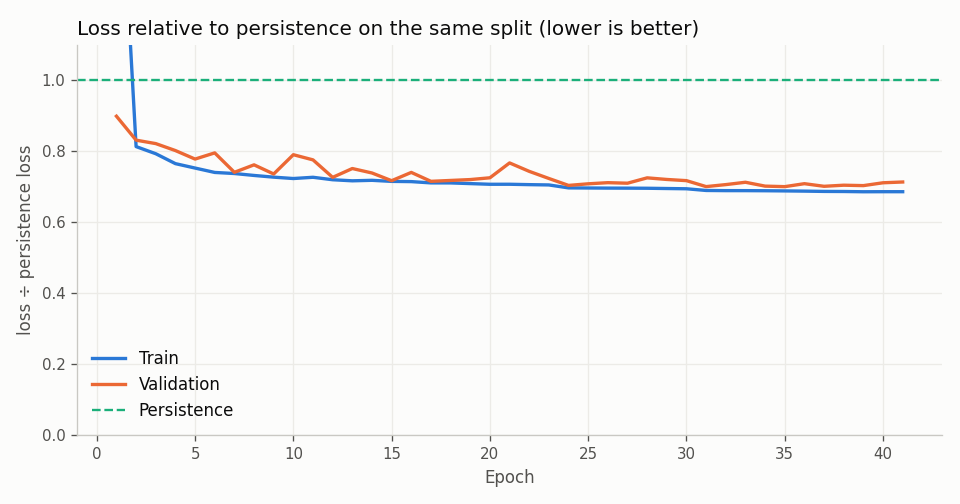
\includegraphics[width=\columnwidth]{loss_curve.png}}
\caption{Training and validation loss per epoch for the final model (Run 3), normalized relative to the Persistence baseline error evaluated on the identical split. Both curves rapidly drop below 1.0 (indicating immediate superiority over persistence) and converge near $0.69\times$--$0.70\times$ persistence loss without overfitting.}
\label{fig:loss_curve}
\end{figure}

\begin{figure*}[t]
\centering
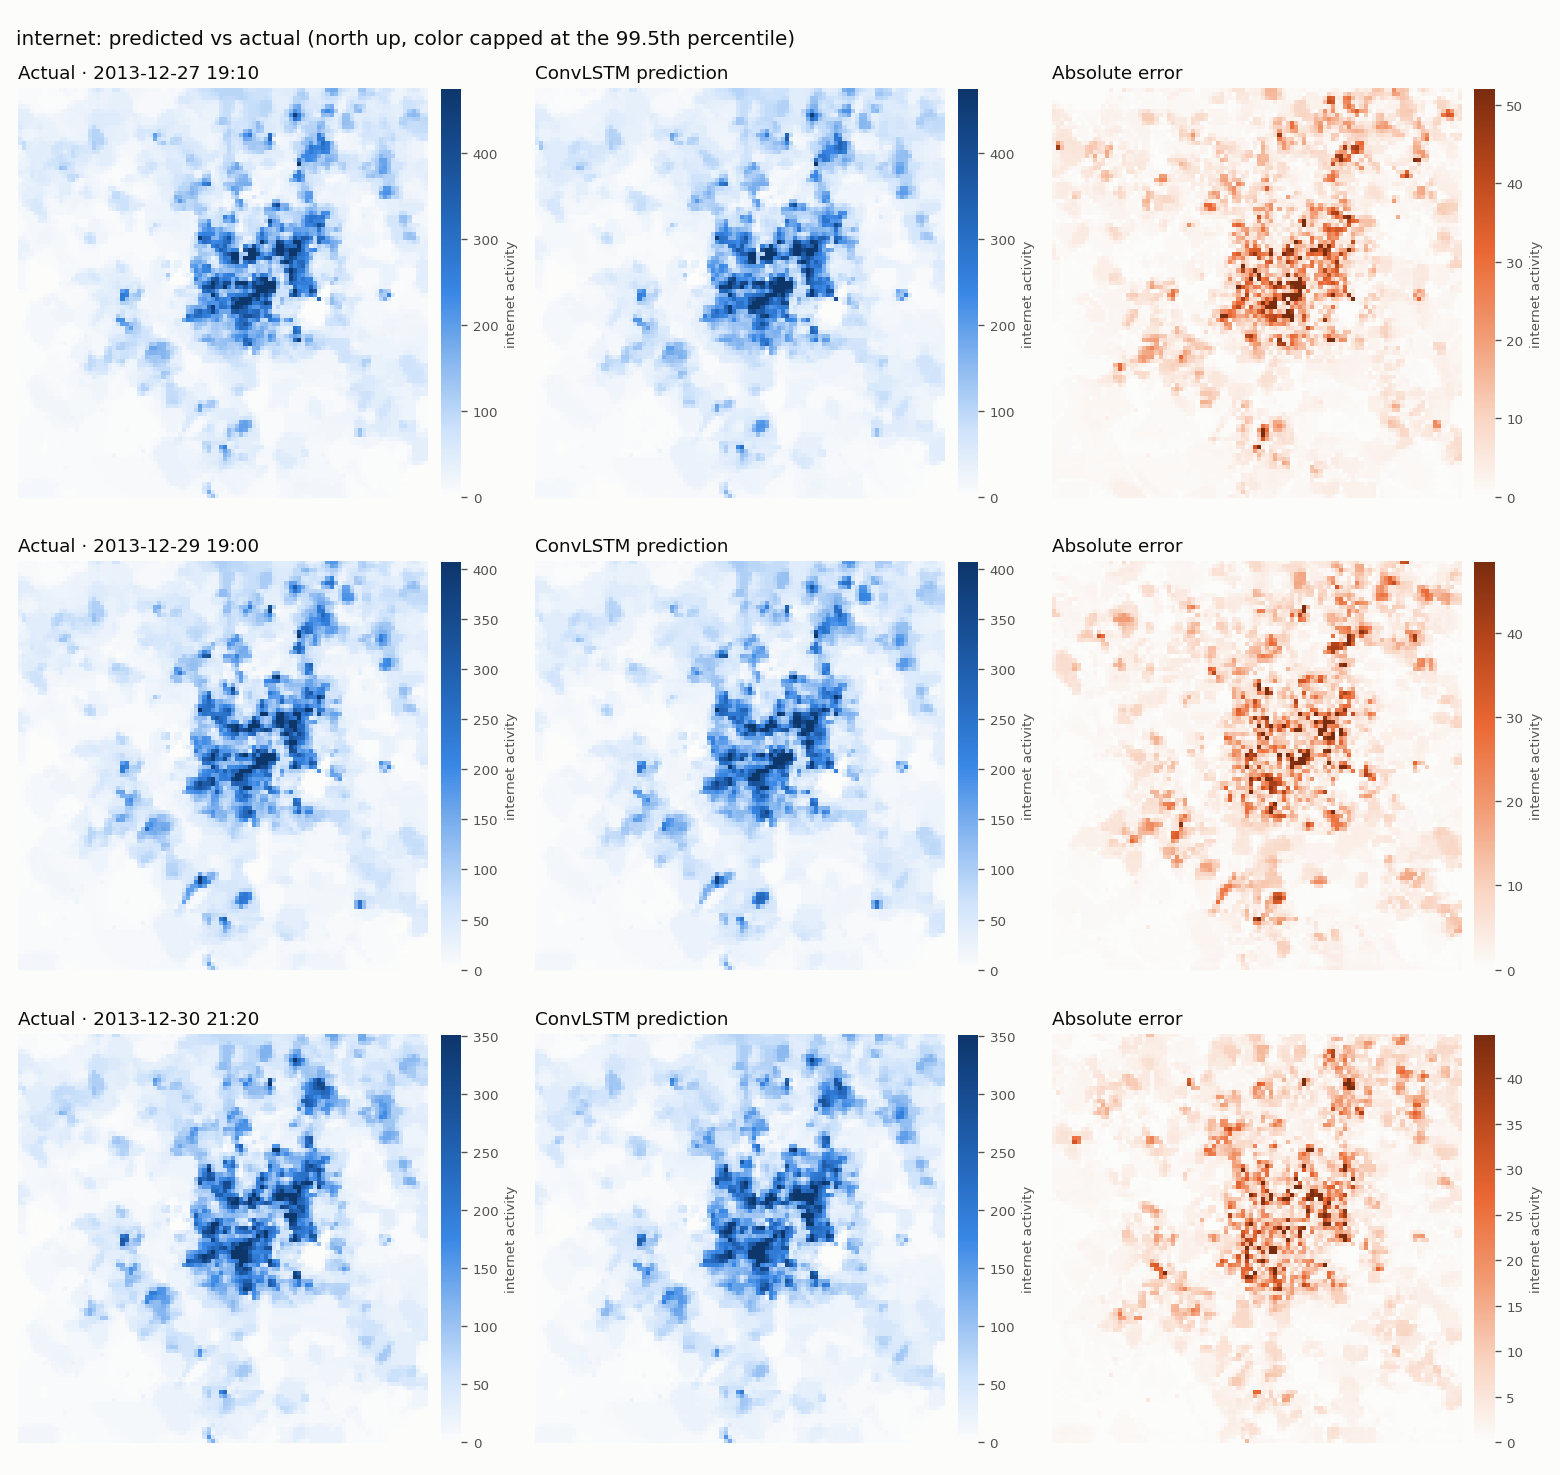
\includegraphics[width=0.98\textwidth]{heatmaps.png}
\caption{Spatial verification across Milan at three distinct test evaluation timestamps (2013-12-27 19:10, 2013-12-29 19:00, and 2013-12-30 21:20). Columns display Ground Truth traffic, ConvLSTM prediction, and Absolute Error maps. Coordinates represent the $100 \times 100$ grid with north at the top.}
\label{fig:heatmaps}
\end{figure*}

\begin{figure}[htbp]
\centerline{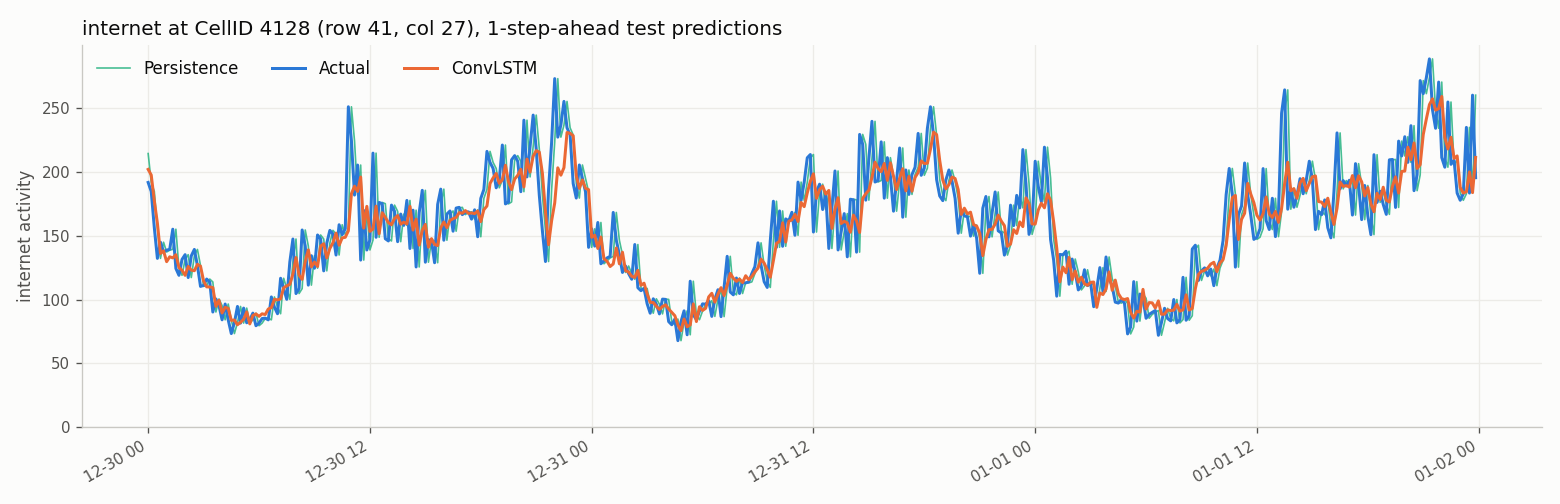
\includegraphics[width=\columnwidth]{cell_timeseries.png}}
\caption{Continuous 1-step-ahead prediction time series for high-activity urban cell ID 4128 across the final three days of the test horizon (December 30, 2013 to January 1, 2014), tracking ground truth (blue), ConvLSTM prediction (orange), and Persistence (green).}
\label{fig:cell_timeseries}
\end{figure}

The proposed ConvLSTM (Run 3) achieves the best performance across all metrics. Key observations:
\begin{enumerate}
    \item \textbf{Superiority Over Persistence:} ConvLSTM outperforms persistence by \textbf{9.80\% in RMSE}, \textbf{12.79\% in MAE}, and \textbf{15.73\% in MAPE}. Because telecommunications traffic changes slowly over a single 10-minute step, persistence represents an extraordinarily stringent baseline. Beating it by double digits in MAE and MAPE confirms that the network extracts genuine spatial diffusion and temporal momentum rather than passively replicating the most recent observation.
    \item \textbf{Window Mean Lags Trends:} The Window Mean baseline performs worse than Persistence (RMSE 10.3727 vs. 9.3922). Simple temporal averaging introduces a phase lag during periods of rapid traffic ramp-up or decay.
    \item \textbf{Failure of Seasonal Baselines:} Seasonal Daily (RMSE 27.45) and Seasonal Weekly (RMSE 57.01) baselines exhibit massive error rates. The test period coincides with the Christmas and New Year holiday fortnight (Dec 23 to Jan 1), during which business districts emptied, university campuses closed, and holiday mobility diverged drastically from prior working weeks. The ConvLSTM successfully adapts to these anomalous holiday regimes because its 1-hour input captures instantaneous real-time conditions rather than relying rigidly on stale historical profiles.
\end{enumerate}

\subsection{Analysis of Convergence and Generalization}
Fig.~\ref{fig:loss_curve} plots the training and validation loss progression normalized by the persistence error computed over each respective split. In Run 1, raw validation loss appeared lower than training loss (order $10^{-6}$), raising initial concerns of data leakage. However, domain analysis revealed that mid-December traffic is intrinsically smoother than November traffic; even the naive persistence baseline yields $1.64\times$ lower error during validation than during training. 

By scaling training and validation losses by their respective split-specific persistence baselines, Fig.~\ref{fig:loss_curve} demonstrates that:
\begin{itemize}
    \item Both training and validation curves track almost identically, reaching $0.688\times$ and $0.700\times$ persistence loss at the best epoch (epoch 35).
    \item The absence of a divergence gap between normalized training and validation loss provides empirical proof that the architecture generalizes stably without overfitting.
\end{itemize}

\subsection{Ablation: The Impact of Logarithmic Scaling}
A central finding of this investigation is the role of variance-stabilizing normalization:
\begin{itemize}
    \item In Run 1, min-max scaling squeezed over 95\% of cell activities near 0 due to extreme peak outliers in the city center. This reduced the MSE training loss to $\approx 6 \times 10^{-6}$, starving the optimizer of strong gradient feedback.
    \item In Run 2, standard $z$-score scaling restored gradients ($\text{loss} \approx 10^{-2}$) and allowed \texttt{ReduceLROnPlateau} to function effectively. However, test RMSE rose slightly from 8.4745 to 8.6032.
    \item In Run 3, applying $\log(1+x)$ prior to standardization produced the definitive breakthrough. Cellular traffic exhibits a heavy right tail (log-normal characteristics). The logarithmic transformation compresses high-magnitude dynamic ranges and emphasizes relative percentage errors across peripheral and suburban cells. Consequently, MAPE dropped from 11.987\% (Run 1) and 12.319\% (Run 2) to \textbf{10.585\% (Run 3)}---a relative percentage accuracy improvement of \textbf{11.7\%} with no degradation in RMSE.
\end{itemize}

\subsection{Spatial and Temporal Qualitative Inspection}
Fig.~\ref{fig:heatmaps} illustrates the spatial fidelity of the predicted traffic maps against ground truth across three distinct test timestamps. The ConvLSTM captures the global structure of Milan: the dense core around the Duomo, secondary traffic nodes around the Porta Garibaldi and Centrale railway stations, and major ring roads. The absolute error maps confirm that prediction residuals are confined primarily to extreme central peaks, while peripheral suburban neighborhoods exhibit near-zero residual variance.

Fig.~\ref{fig:cell_timeseries} examines the temporal tracking performance on Cell ID 4128 (a bustling urban cell) through New Year's Eve 2013. While the persistence baseline constantly lags behind rapid inflection points by exactly one time step, the ConvLSTM smoothly filters out stochastic single-step noise and tracks diurnal inflection peaks accurately.

\section{Engineering Considerations and Lessons Learned}
Scaling deep spatio-temporal models to 20\,GB telecommunications datasets under constrained compute environments presents significant systems challenges:
\begin{enumerate}
    \item \textbf{Out-of-Core Preprocessing:} Memory-mapping the $(8928, 5, 100, 100)$ tensor via \texttt{numpy.memmap} eliminated out-of-memory crashes on host systems with limited RAM, allowing PyTorch multi-process workers to stream slices on demand.
    \item \textbf{Time Budget and Resumption:} Under Kaggle's 12-hour session limit, a time-budget monitor halts training gracefully at 8.5 hours, serializing \texttt{last\_checkpoint.pt} to guarantee evaluation execution and enable multi-session continuation.
    \item \textbf{Relative Early Stopping Threshold:} Relying on raw floating-point loss improvements kept Run 1 active for 10 redundant epochs due to negligible fluctuations in the 7th decimal place. Enforcing a relative threshold ($\Delta_{\text{rel}} \ge 0.1\%$) shortened training time by 28 minutes while yielding superior final weights.
\end{enumerate}

\section{Conclusion and Future Work}
In this work, we developed and benchmarked a Spatio-Temporal Convolutional LSTM network for short-term cellular internet traffic forecasting across the entire metropolitan area of Milan. By combining a two-layer ConvLSTM backbone with cyclical calendar encodings, a residual convolutional head, and logarithmic variance stabilization, the proposed architecture predicts city-wide cellular demand 10 minutes ahead with an RMSE of 8.4722, MAE of 3.7802, and MAPE of 10.585\%. The model outperforms the formidable persistence baseline by 9.8\% in RMSE and 15.7\% in MAPE during an anomalous holiday test period, demonstrating robust generalization without data leakage.

Future extensions will explore:
\begin{itemize}
    \item \textbf{Multi-Horizon Sequence-to-Sequence:} Incorporating an encoder-decoder ConvLSTM structure to forecast multiple time steps ahead ($T_{\text{out}} \in \{3, 6, 12\}$) without recursive error compounding.
    \item \textbf{Multimodal Feature Fusion:} Leveraging SMS and telephony activity channels as cross-modal covariates to predict internet surges.
    \item \textbf{Graph Wavelet Networks:} Comparing regular grid convolutions with graph-based message passing conditioned on the irregular Voronoi geometries of real-world cell towers.
\end{itemize}

\begin{thebibliography}{00}
\bibitem{b1} C. Zhang, P. Patras, and H. Haddadi, ``Deep learning in mobile and wireless networking: A survey,'' \textit{IEEE Commun. Surveys Tuts.}, vol. 21, no. 3, pp. 2224--2287, 3rd Quart., 2019.
\bibitem{b2} J. Wang, J. Tang, Z. Xu, Y. Wang, G. Xue, X. Zhang, and D. Yang, ``Spatiotemporal modeling and prediction in cellular networks: A big data perspective,'' in \textit{Proc. IEEE INFOCOM}, 2017, pp. 1--9.
\bibitem{b3} M. Z. Shafiq, L. Ji, A. X. Liu, and J. Wang, ``A first look at cellular machine-to-machine traffic: Large scale measurement and characterization,'' in \textit{Proc. ACM SIGMETRICS}, 2012, pp. 65--76.
\bibitem{b4} X. Shi, Z. Chen, H. Wang, D. Y. Yeung, W. K. Wong, and W. C. Woo, ``Convolutional LSTM network: A machine learning approach for precipitation nowcasting,'' in \textit{Proc. Adv. Neural Inf. Process. Syst. (NeurIPS)}, 2015, pp. 802--810.
\bibitem{b5} C. Qiu, Y. Zhang, Z. Feng, P. Zhang, and S. Cui, ``Spatio-temporal wireless traffic prediction with recurrent neural network,'' \textit{IEEE Wireless Commun. Lett.}, vol. 7, no. 4, pp. 554--557, Aug. 2018.
\bibitem{b6} J. L. Wu, Y. Liu, C. Shen, and X. Guan, ``A hybrid deep learning framework for cellular traffic prediction,'' \textit{IEEE Trans. Cogn. Commun. Netw.}, vol. 7, no. 2, pp. 382--394, Jun. 2021.
\bibitem{b7} S. Hochreiter and J. Schmidhuber, ``Long short-term memory,'' \textit{Neural Comput.}, vol. 9, no. 8, pp. 1735--1780, Nov. 1997.
\bibitem{b8} J. Zhang, Y. Zheng, and D. Qi, ``Deep spatio-temporal residual networks for citywide crowd flows prediction,'' in \textit{Proc. AAAI Conf. Artif. Intell.}, 2017, pp. 1655--1661.
\bibitem{b9} Y. Wang, M. Long, J. Wang, Z. Gao, and P. S. Yu, ``PredRNN: Recurrent neural networks for predictive learning using spatiotemporal LSTMs,'' \textit{IEEE Trans. Pattern Anal. Mach. Intell.}, vol. 45, no. 6, pp. 7476--7492, Jun. 2023.
\bibitem{b10} L. Zhao, Y. Song, C. Zhang, Y. Liu, P. Wang, T. Lin, M. Deng, and H. Li, ``T-GCN: A temporal graph convolutional network for traffic prediction,'' \textit{IEEE Trans. Intell. Transp. Syst.}, vol. 21, no. 9, pp. 3848--3858, Sep. 2020.
\bibitem{b11} Telecom Italia, ``Telecommunications - SMS, Call, Internet - MI,'' Harvard Dataverse, doi:10.7910/DVN/EGZHFV, 2015.
\bibitem{b12} G. Barlacchi, M. De Nadai, R. Larcher, A. Casella, C. Chitic, G. Torrisi, F. Tucci, M. Vescovi, A. Pentland, and B. Lepri, ``A multi-source dataset of urban life in the city of Milan and the Province of Trentino,'' \textit{Sci. Data}, vol. 2, Art. no. 150055, Oct. 2015.
\end{thebibliography}

\end{document}
